\documentclass{article}
\usepackage{blindtext}
\usepackage[utf8]{inputenc}
\usepackage{amsmath,bm}
\usepackage{amstext}
\usepackage{amsfonts}
\usepackage{amsmath}
\usepackage{epsfig}
\usepackage{CTEX}
\usepackage[colorlinks,linkcolor=blue]{hyperref}

\title{Homework 3实验报告}
\author{181860066 牛铭杨}

\begin{document}
\maketitle
\numberwithin{equation}{section}
\section{实验设置}
    本次实验我按照要求使用Pytorch搭建了一个卷积神经网络架构,对MNIST数据集进行预测。

    首先仿照实例代码读入训练集和测试集数据,然后自定义class Net来定义神经网络架构,基本架构如图。
    之后定义损失函数和优化算法,这里我用了损失函数nll\_loss,优化算法SGD和Adam,并统计了训练损失和验证损失还有准确率。
    \begin{figure}
        \centering
        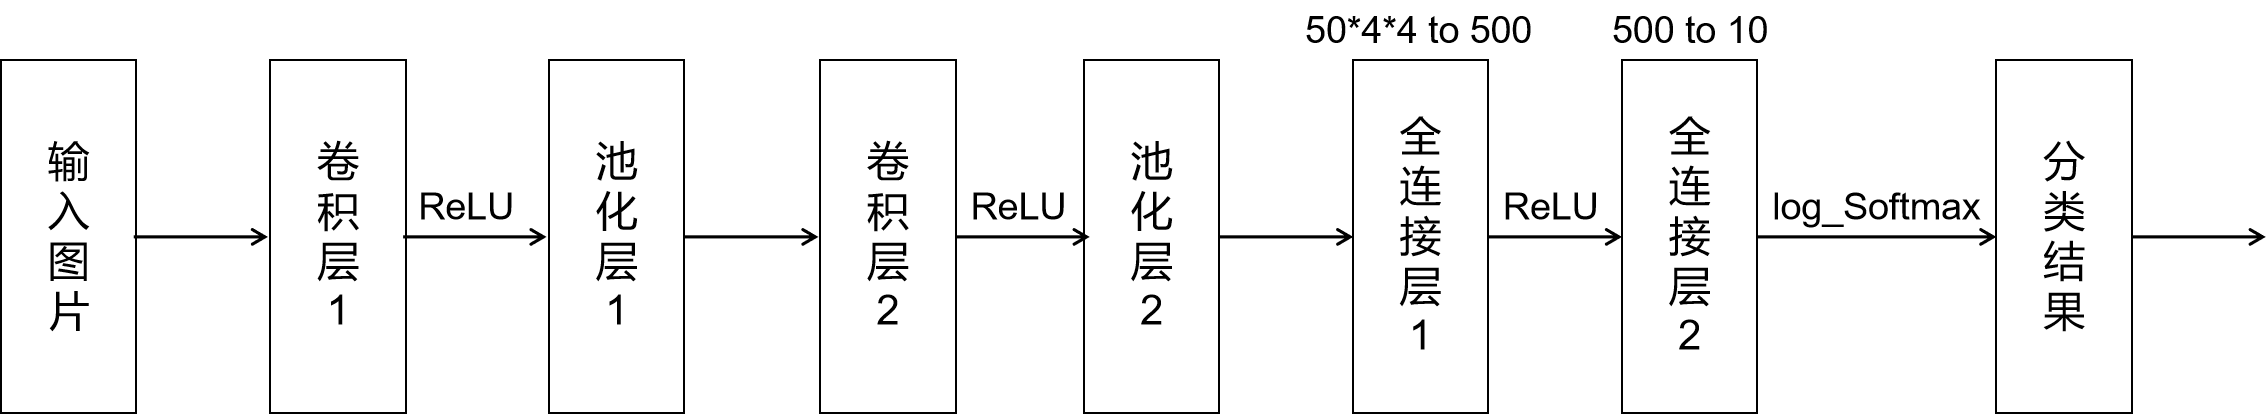
\includegraphics[width=.7\textwidth]{network_architecture.png}
        \caption{神经网络架构}
    \end{figure}
    \\\\
\section{实验结果}
    使用的优化算法、训练批次和学习率对验证集上准确率的影响如图。训练批次共10批,使用了SGD和Adam
    算法优化,并调整学习率和动量得到坐标图。

    \begin{figure}
        \centering
        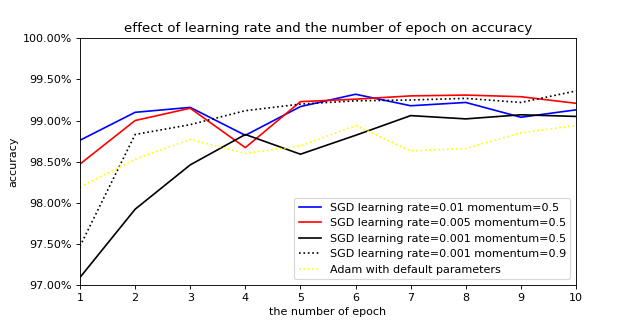
\includegraphics[width=.7\textwidth]{learning rate effect.png}
        \caption{各参数对准确率的影响}
    \end{figure}

    可以看出,随着训练批次的增加,准确率呈上升趋势,但是最后反而会有一定下降,这是由于过拟合,
    而学习率则是和动量一起对准确率造成影响。学习率大时可以较早收敛,学习率小时收敛慢,但是更加稳定。

    训练损失和验证损失随训练批次的变化如图3.
    \begin{figure}
        \centering
        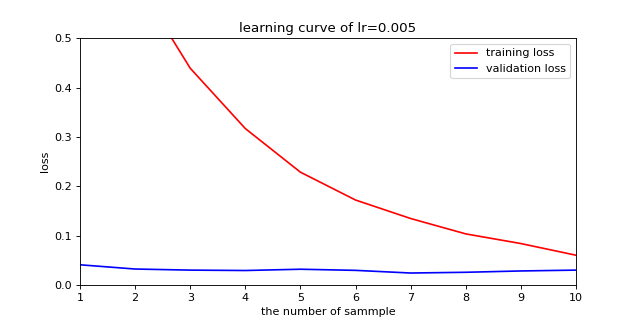
\includegraphics[width=.7\textwidth]{learni curve.png}
        \caption{训练损失和验证损失随训练批次的变化}
    \end{figure}
    
\end{document}
